\documentclass[conference]{IEEEtran}

\usepackage{blindtext}
\usepackage{graphicx}
\usepackage{hyperref}
%\usepackage{caption}
%\usepackage{subcaption}

\usepackage{cite}
% Loading the cite package will
% result in citation numbers being automatically sorted and properly
% "compressed/ranged". e.g., [1], [9], [2], [7], [5], [6] without using
% cite.sty will become [1], [2], [5]--[7], [9] using cite.sty. cite.sty's
% \cite will automatically add leading space, if needed. 

% correct bad hyphenation here
\hyphenation{op-tical net-works semi-conduc-tor}


\begin{document}

% can use linebreaks \\ within to get better formatting as desired
\title{StudyPal: A Website for Study Groups}

\author{\IEEEauthorblockN{James Beavers}
\IEEEauthorblockA{Department of Computer Science\\
North Carolina State University\\
Raleigh, North Carolina, USA\\
jjbeaver@ncsu.edu}
\and
\IEEEauthorblockN{Anthony Elliott}
\IEEEauthorblockA{Department of Computer Science\\
North Carolina State University\\
Raleigh, North Carolina, USA\\
anthony\_elliott@ncsu.edu}}


\maketitle


\begin{abstract}
Current university students form study groups with peers to help prepare for exams or work through assignments together.
Students often form study groups only with people they know very well from face-to-face contact.
We developed a prototype website called StudyPal to facilitate the creation and organization of study groups.
We predict how long experts should take to complete three primary tasks within StudyPal using the Keystroke-Level Model and conducted an empirical evaluation of 4 people to assess the accuracy of the predictions.
\end{abstract}

\IEEEpeerreviewmaketitle



\section{Introduction}
StudyPal is a website we designed and created to help university students form study groups for their classes.

%todo: might be better to merge these subsections later, I created them just to make sure I got everything

\subsection{Task Domain}
Students often form study groups for a specific class in which they help each other with exam preparation, readings, or assignments.
These study groups are formalized meetings set up ahead of time, in contrast to unplanned meetings.
Meeting length can vary from one hour to several hours.
Group sizes are typically small, with 2-5 participants.
Groups often consist of systematically going through a study guide for the class, either provided by the class instructor or created by the group participants.


\subsection{Target Users}
StudyPal is intended for use by both undergraduate and graduate students at North Carolina State University (NCSU).
If successful at NCSU then we plan to extend StudyPal to students at other universities.
StudyPal currently only uses the English language and thus only expected to be used by English-speaking students.


\subsection{Representative Scenarios}

\subsubsection{Joining a Group}
Users enter the website and enter their user information to create an account.
After logging in to the website, the user inputs their class schedule and selects which of their current classes they are interested in joining a study group for.
StudyPal then displays all current study groups for that class that are still looking for more members.
The user scrolls through the list of groups and selects one to view the details of.
The user looks at the desired qualifications of group members and hits 'Apply' if interested in joining the group.
The group creator then sees that someone has requested group access and can choose to accept or reject this applicant.

If there are no groups for this class or the user does not want to join any of the existing groups then they can create a group themselves.

\subsubsection{Creating a Group}
A user who wants to create a study group first logs in to the StudyPal website, and hits the 'Create a Group' button displayed on multiple pages.
They enter basic information about the group, such as course and frequency of meetings.
Fields such as time and place can be skipped if not yet decided on.
The user then enters qualifications such as 'have read all chapters', or 'attends all classes' that every group member should have.
This creates the group and the user waits for other students to see this group and apply to join.
The user can then accept or reject students who apply to join the group.

\subsubsection{Group Notifications}
%todo: put more detail here
%todo: will we implement a better notification system (e.g. button for 'Email all participants')?
Each participant in a StudyPal group can see all other email addresses of the other participants and can use email to send updates to the group.



\section{Related Work}
A description of related work, including related systems and papers from the academic literature. Related work encompasses interactive systems in the task domain, interactive systems for related tasks, and general HCI research. Reference any external material you rely on including papers, books, commercial systems, Web pages, and so forth. Highlight the influences of this material on your work. 

\emph{The report demonstrates depth of knowledge of the area, in both theoretical and practical terms.}




\section{System Design}
A description of the design of the system. You should also describe its evolution through the design process, along with the influence of user testing and formative evaluation techniques on the design decisions you made. Artifacts (e.g., notes from interviews, sketches, early mock-ups, etc.) maybe included in the written report as an appendix. 

\emph{The system clearly reflect users' concerns, as demonstrated by the extensive use of relevant HCI techniques for discovery and design. User feedback has been taken into account in the design, as illustrated by specific examples (e.g., quotes from users and descriptions of design changes). Best practices in HCI development have been followed.}

% user interviews
% sketches
% development
% user feedback (where I'm the user)

We wanted to create a very simple user interface that could be quickly used by an expert.
We also wanted our website to be easy to use for novices, that is, we wanted novices to be able to complete basic tasks in the website without requiring outside help.
The specific tasks that we wanted to support are joining an existing group, creating a new group, and sending notifications to the group members.

We first started by interviewing several students who have previously used study groups for their classes in order to better determine the scope of our system.

After extracting requirements from the interviews, we sketched mockups of the website using pencil and paper.
%todo These sketches are included in ____
The sketches helped us identify challenges that we would face.

One challenge was how to integrate the user's schedule into our system.
One user said that ``even though courses appear on my schedule, I don't always have to go to them and would still be available to meet.''
This highlights the issue that a schedule may not be accurate for all users and thus we don't want to hide groups that meet during these times in case the user actually wants to attend those meetings.
However, many users would \emph{not} want to see groups that conflict with classes.
To resolve this issue we decided to indicate conflicting times by dimming the background color of those groups when trying to find a group.
%todo implement the dimming


In interviews, one participant said that ``the level of distraction increases with the number of people in the group.''
The same participant said that 5 study group members was the upper limit for productivity, however, other interview participants said they frequently had study groups with around 5 members.
This shows that a generally small group is more desirable, but further research is needed to see how group size impacts study group results.
We decided to prominently display the current group size for potential applicants so that they could make their own decision if they wanted to join a group with 5 or more members.

Another issue was group member requirements.
We discovered in interviews that study groups are usually formed via personal connections and many subjective decisions were made to determine who to invite to the group.
One participant said that all study group members ``need a common background'', for example, each member should have at least passing familiarity with each section of material.
Defining this 'common background' is an example of such subjective decisions.
We did not want to implement complex qualification algorithms without basing decisions on solid research, so we allow group leaders to create subjective qualifications and decide themselves.
Group leaders enter desired qualifications of group members, other students can apply after reading through the qualifications, and then the leader reviews each application and can either accept or reject them.


Frequency of study groups is another issue that emerged from the interviews.
Some students typically formed a study group that only met once per exam while others met on a regular basis.
We extracted discrete intervals of once, weekly, and monthly for study groups.





\section{Analytical Interface Evaluation}
%An analytical evaluation of your interface, using modeling techniques you judge to be most appropriate. 
 
%\emph{A specific analytical technique modeling technique is correctly applied; its choice is well-justified and the results are explained in detail. The analytical technique is such that it provides predictions or explanations of actual user performance. Insights from the analytical evaluation are discussed. The relevance of the modeling results to usability are made clear.}

% use the KLM
 
In this section we provide an analytical evaluation of StudyPal.
Specifically, we describe why we chose the KLM model\cite{Card:KLM}, how we applied the model to three use cases of StudyPal, and what these results mean in terms of the usability of StudyPal.

\subsection{Why KLM?}
The Keystroke-Level Model (KLM) \cite{Card:KLM} is a simple model to predict how long expert users will need to perform a given task on a computer system.
Limiting the scope of our analysis to expert users who rarely make mistakes makes sense for initial predictions.
As more people use StudyPal, exploring alternative methods could add more value with more accurate predictions.

One such alternative is ACT-R\cite{Anderson:ACT-R} which offers more accurate predictions, but takes much more effort.
Another alternative is NGOMSL\cite{Kieras:NGOMSL} which incorporates learning in order to extend the scope of the predictions

% explain why using the KLM
 % sufficient for our needs
 % a more detailed analysis would benefit from the NGOMSL because it factors in learning time
 % KLM limitations: 
   % errors
   % learning
   % functionality
   % recall
   % concentration
   % fatigue
   % acceptability
 % we don't care much about the missing pieces above (except learning)

\subsection{Application of KLM}
We describe how we applied the KLM to the three main use cases of StudyPal.
All three use cases, or tasks, assume that the user is already logged in to StudyPal and located at the home page.

\subsubsection{Joining a Group}
The user must first click on the ``List all groups'' button, then click on a group to display group details, read the displayed information and then hit 'Apply'.

\paragraph{List all groups:}
This requires the user to home (H) their hand to the mouse, point (P) at the button with the mouse, and click (K) the button using the left mouse button.
The user then waits for StudyPal to respond (R).

In the KLM, this is encoded as: \emph{HPKR}.

The KLM predicts that homing takes 0.4 seconds, pointing takes 1.1 seconds, and the key press takes 0.2 seconds.
This results in a time of 1.7 seconds to list all existing groups, assuming negligible system response time.

\paragraph{Display group details:}
Now that the system has displayed all existing groups, the user must find one they are interested in joining.
The user should already have their hand on the mouse from the previous action, so we will not factor a homing action in here.
This task requires the user to point (P) with their mouse to the name of the group they want to join, click (K), and then wait for the system to respond (R).

In the KLM, this is encoded as: \emph{PKR}.

The KLM predicts the pointing to take 1.1 seconds, the button press to take 0.2 seconds, and the system response time is assumed to be negligible.
This results in a time of 1.3 seconds to display the details of a group.

\paragraph{Apply:}
Once displayed with the group details, the user needs to hit the 'Apply' button to submit their application to the group leader.
The user should already have their hand on the mouse from the previous action, so we will not factor a homing action in here.
This task requires the user to point (P) with their mouse to the 'Apply' button, click (K), and then wait for the system to respond (R).

In the KLM, this is encoded as: \emph{PKR}.

The KLM predicts the pointing to take 1.1 seconds, the button press to take 0.2 seconds, and the system response time is assumed to be negligible.
This results in a time of 1.3 seconds to apply to a group.

The user must now wait for the study group leader to review their application before being allowed formal entrance into the group.

\textbf{Total time:}
Combining the above encodings we get \emph{HPKRPKRPKR} in the KLM and a total time of 4.3 seconds to list all of the existing groups.


\subsubsection{Creating a Group}
The user must first click on the ``Create group'' button, enter the group title, enter the course name, select the frequency of meeting, and then submit the form.
Other optional information fields exist but we exclude them from this model as they are not part of the minimum action set needed to create a group.

\paragraph{Click ``Create group'':}
From the home page, the user needs to click the `Create group' button.
This requires the user to home (H) their hand to the mouse, point (P) at the button with the mouse, and click (K) the button using the left mouse button.
The user then waits for StudyPal to respond (R).

In the KLM, this is encoded as: \emph{HPKR}.

The KLM predicts that homing takes 0.4 seconds, pointing takes 1.1 seconds, and the key press takes 0.2 seconds.
This results in a time of 1.7 seconds to display the form for group creation, assuming negligible system response time.

\paragraph{Enter group title:}
After the group creation form has been displayed, the user must enter a title for this group.
For the purposes of this model we will assume that the average group name consists of two words, and that each word consists of an average length of five characters\footnote{http://www.wolframalpha.com/input/?i=average+word+length}.
In totaling the characters, we find that there are 10 characters plus one delimiter such as a space or dash resulting in an average group title length of 11 characters.

To enter this, the user must first point (P) with the mouse to the input field, click (K) to select the input field, home (H) their hands to the keyboard, enter one word of 5 characters, enter a space, and enter another word of 5 characters.
We have spaced the following encoding to represent these actions.

This results in a KLM encoding of \emph{PKH MKKKKK K MKKKKK}.
The KLM predicts that pointing will take 1.1 seconds, each of the 12 key presses will take 0.2 seconds, the homing will take 0.4 seconds, and the single act of mental preparation will take 1.35 seconds.
This results in a total time of 4.89 seconds to enter the title of the group.

\paragraph{Enter course name:}
After entering the group title, the user must enter the name of the course this group will be studying.
Most university courses can be represented with a three letter department indicator (e.g. CSC for Computer Science) and a three digit course number (e.g. 554).

To enter this, the user can home (H) to the keyboard, hit the TAB button (K) to move to from the title input form to the course name input form, type the three letter department abbreviation (KKK), type a space (K), and finally type the three digit course number (KKK).

Combining these encodings with needed mental preparation results in a KLM encoding of \emph{HKMKKKKMKKK}.
The KLM predicts that the homing act will take 0.4 seconds, each of the 8 key presses will take 0.2 seconds, and the mental preparation will take 1.35 seconds.
This results in a total time of 3.35 seconds to enter the course name.

\paragraph{Select frequency:}
After entering the course name, the user must select one of three frequencies (meet once, meet weekly, or meet monthly) from a drop down menu.
We select `Once' by default as we expect this to be the most common of the three.
If the user wants to keep the default frequency of `Once' then this entire step can be skipped.

Otherwise, the user will need to home (H) their hands to the keyboard, hit the TAB button (K) to select the frequency drop down menu, and hit the down arrow key twice (KK) to advance from `Once' to `Weekly' to `Monthly'.

This results in a KLM encoding of \emph{HKMKK}.
The KLM predicts that the homing act will take 0.4 seconds, each of the 3 key presses will take 0.2 seconds, and the mental preparation will take 1.35 seconds.
Thus frequency selection is predicted to take a total time of 2.35 seconds.

\paragraph{Submit form:}
After entering all required information, the user must submit the form by hitting the ENTER button.

The user must home (H) to the keyboard, hit the ENTER key (K), and wait for the system to respond (R).
This results in a KLM encoding of \emph{HKR}.
The KLM predicts that the homing will take 0.4 seconds, the single keypress will take 0.2 seconds, and we assume a negligible system response time.
Thus we predict form submission to take 0.6 seconds.

\textbf{Total time:}
Here we sum the time of each subtask.
Clicking `Create group' is predicted to take 1.7 seconds,
entering the group title should take 4.89 seconds,
entering the course name should take 3.35 seconds,
selecting the frequency should take 2.35 seconds,
and form submission should take 0.6 seconds.

This results in a total time of 12.89 seconds to create a group.


\subsubsection{Send Notification to Group}
%todo implement this in the tool and then apply the KLM.
% Using the same format as I have would be ideal.
% If you want to change the format then go ahead, I just got text on the page in a semblence of logical order. :)


\subsection{Usability Implications}


\section{Empirical Interface Evaluation}
An empirical, formative evaluation of your interface. This should be run with at least four users, classmates or non-classmates. The evaluation records both quantitative and qualitative information. 

\emph{The formative evaluation is well-designed to give information about the usability of the system. It also provides information that allows for comparison with the analytical evaluation; that comparison is made. Results are discussed in enough detail that their generality is clear, suggesting how well the system would work if it could be deployed in the real world and a full-scale empirical evaluation carried out. In other words, it's clear how well the system works.}

% needed in second column of first page if using \IEEEpubid
%\IEEEpubidadjcol

% An example of a floating figure using the graphicx package.
% Note that \label must occur AFTER (or within) \caption.
% For figures, \caption should occur after the \includegraphics.
% Note that IEEEtran v1.7 and later has special internal code that
% is designed to preserve the operation of \label within \caption
% even when the captionsoff option is in effect. However, because
% of issues like this, it may be the safest practice to put all your
% \label just after \caption rather than within \caption{}.
%
% Reminder: the "draftcls" or "draftclsnofoot", not "draft", class
% option should be used if it is desired that the figures are to be
% displayed while in draft mode.
%
%\begin{figure}[!t]
%\centering
%\includegraphics[width=2.5in]{myfigure}
% where an .eps filename suffix will be assumed under latex, 
% and a .pdf suffix will be assumed for pdflatex; or what has been declared
% via \DeclareGraphicsExtensions.
%\caption{Simulation Results}
%\label{fig_sim}
%\end{figure}

% Note that IEEE typically puts floats only at the top, even when this
% results in a large percentage of a column being occupied by floats.


% An example of a double column floating figure using two subfigures.
% (The subfig.sty package must be loaded for this to work.)
% The subfigure \label commands are set within each subfloat command, the
% \label for the overall figure must come after \caption.
% \hfil must be used as a separator to get equal spacing.
% The subfigure.sty package works much the same way, except \subfigure is
% used instead of \subfloat.
%
%\begin{figure*}[!t]
%\centerline{\subfloat[Case I]\includegraphics[width=2.5in]{subfigcase1}%
%\label{fig_first_case}}
%\hfil
%\subfloat[Case II]{\includegraphics[width=2.5in]{subfigcase2}%
%\label{fig_second_case}}}
%\caption{Simulation results}
%\label{fig_sim}
%\end{figure*}
%
% Note that often IEEE papers with subfigures do not employ subfigure
% captions (using the optional argument to \subfloat), but instead will
% reference/describe all of them (a), (b), etc., within the main caption.


% An example of a floating table. Note that, for IEEE style tables, the 
% \caption command should come BEFORE the table. Table text will default to
% \footnotesize as IEEE normally uses this smaller font for tables.
% The \label must come after \caption as always.
%
%\begin{table}[!t]
%% increase table row spacing, adjust to taste
%\renewcommand{\arraystretch}{1.3}
% if using array.sty, it might be a good idea to tweak the value of
% \extrarowheight as needed to properly center the text within the cells
%\caption{An Example of a Table}
%\label{table_example}
%\centering
%% Some packages, such as MDW tools, offer better commands for making tables
%% than the plain LaTeX2e tabular which is used here.
%\begin{tabular}{|c||c|}
%\hline
%One & Two\\
%\hline
%Three & Four\\
%\hline
%\end{tabular}
%\end{table}


% Note that IEEE does not put floats in the very first column - or typically
% anywhere on the first page for that matter. Also, in-text middle ("here")
% positioning is not used. Most IEEE journals use top floats exclusively.
% Note that, LaTeX2e, unlike IEEE journals, places footnotes above bottom
% floats. This can be corrected via the \fnbelowfloat command of the
% stfloats package.



\section{Conclusion}
\blindtext





% if have a single appendix:
%\appendix[Proof of the Zonklar Equations]
% or
%\appendix  % for no appendix heading
% do not use \section anymore after \appendix, only \section*
% is possibly needed

% use appendices with more than one appendix
% then use \section to start each appendix
% you must declare a \section before using any
% \subsection or using \label (\appendices by itself
% starts a section numbered zero.)
%


\appendices
\section{Sketches of Early Design}
\begin{figure}[ht!]
\centering
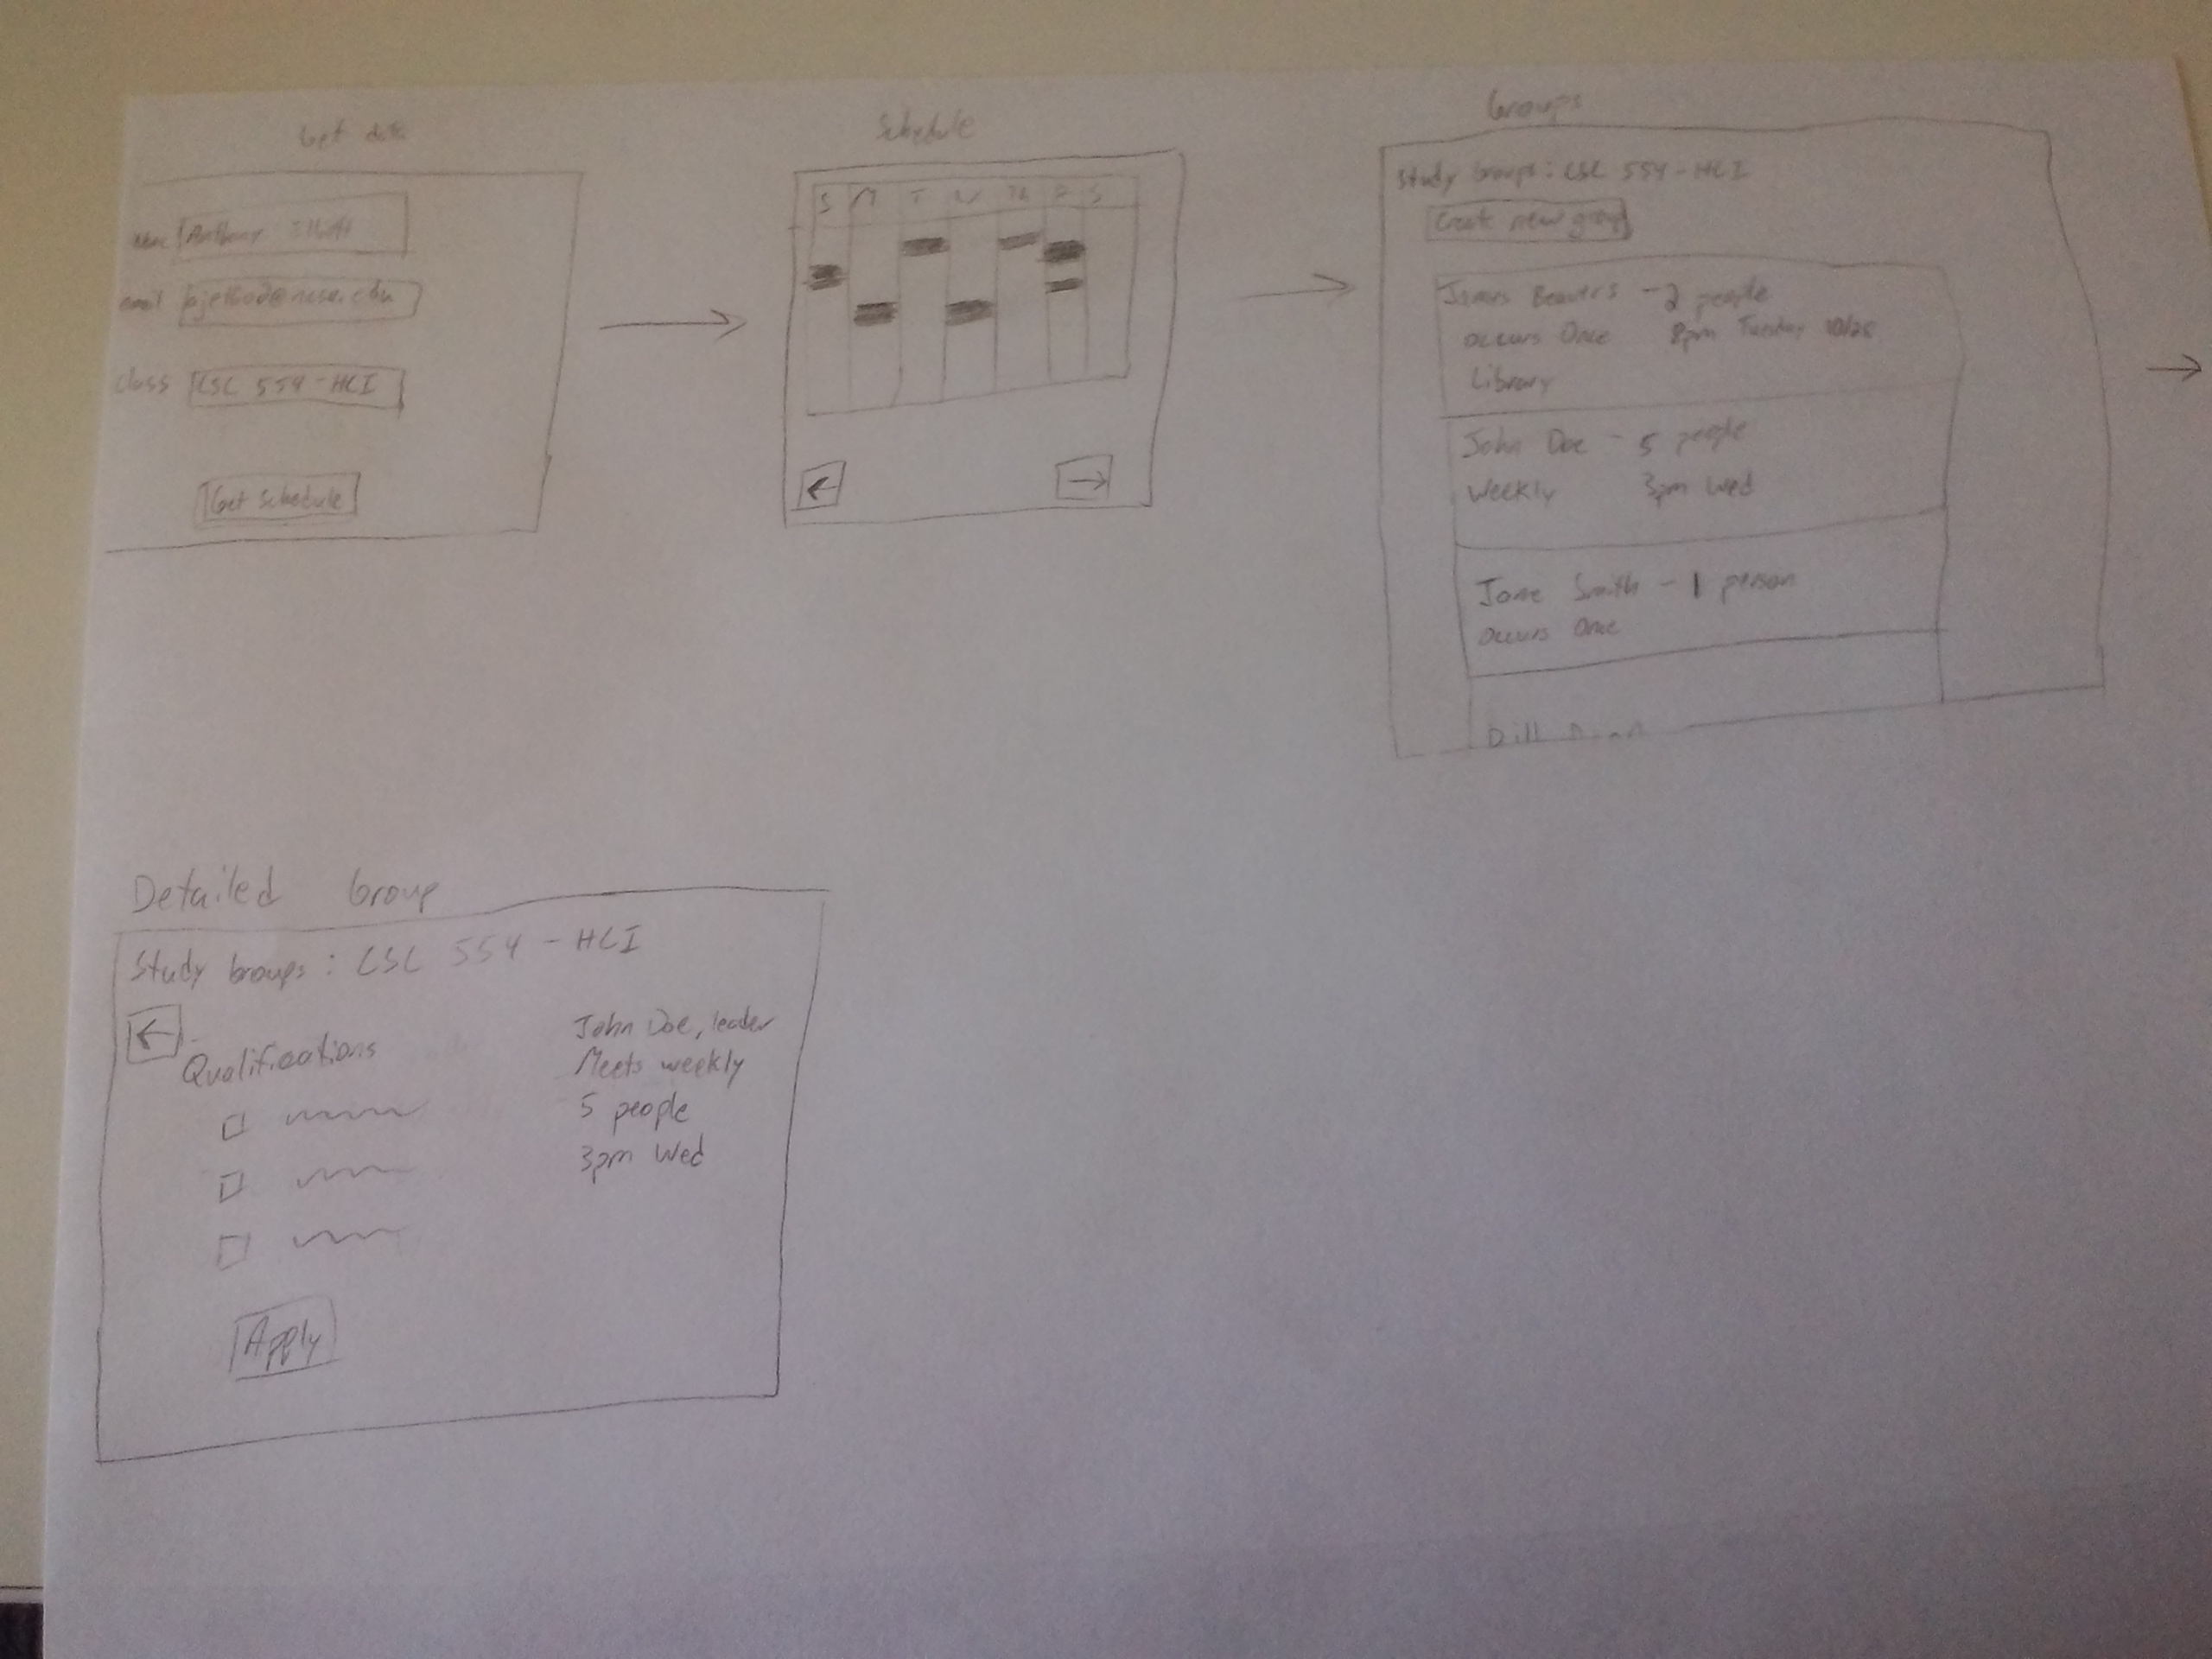
\includegraphics[width=80mm]{figures/flow}
\caption{Shows the flow of the different screens. \label{fig:flow}}
\end{figure}

\begin{figure}[ht!]
\centering
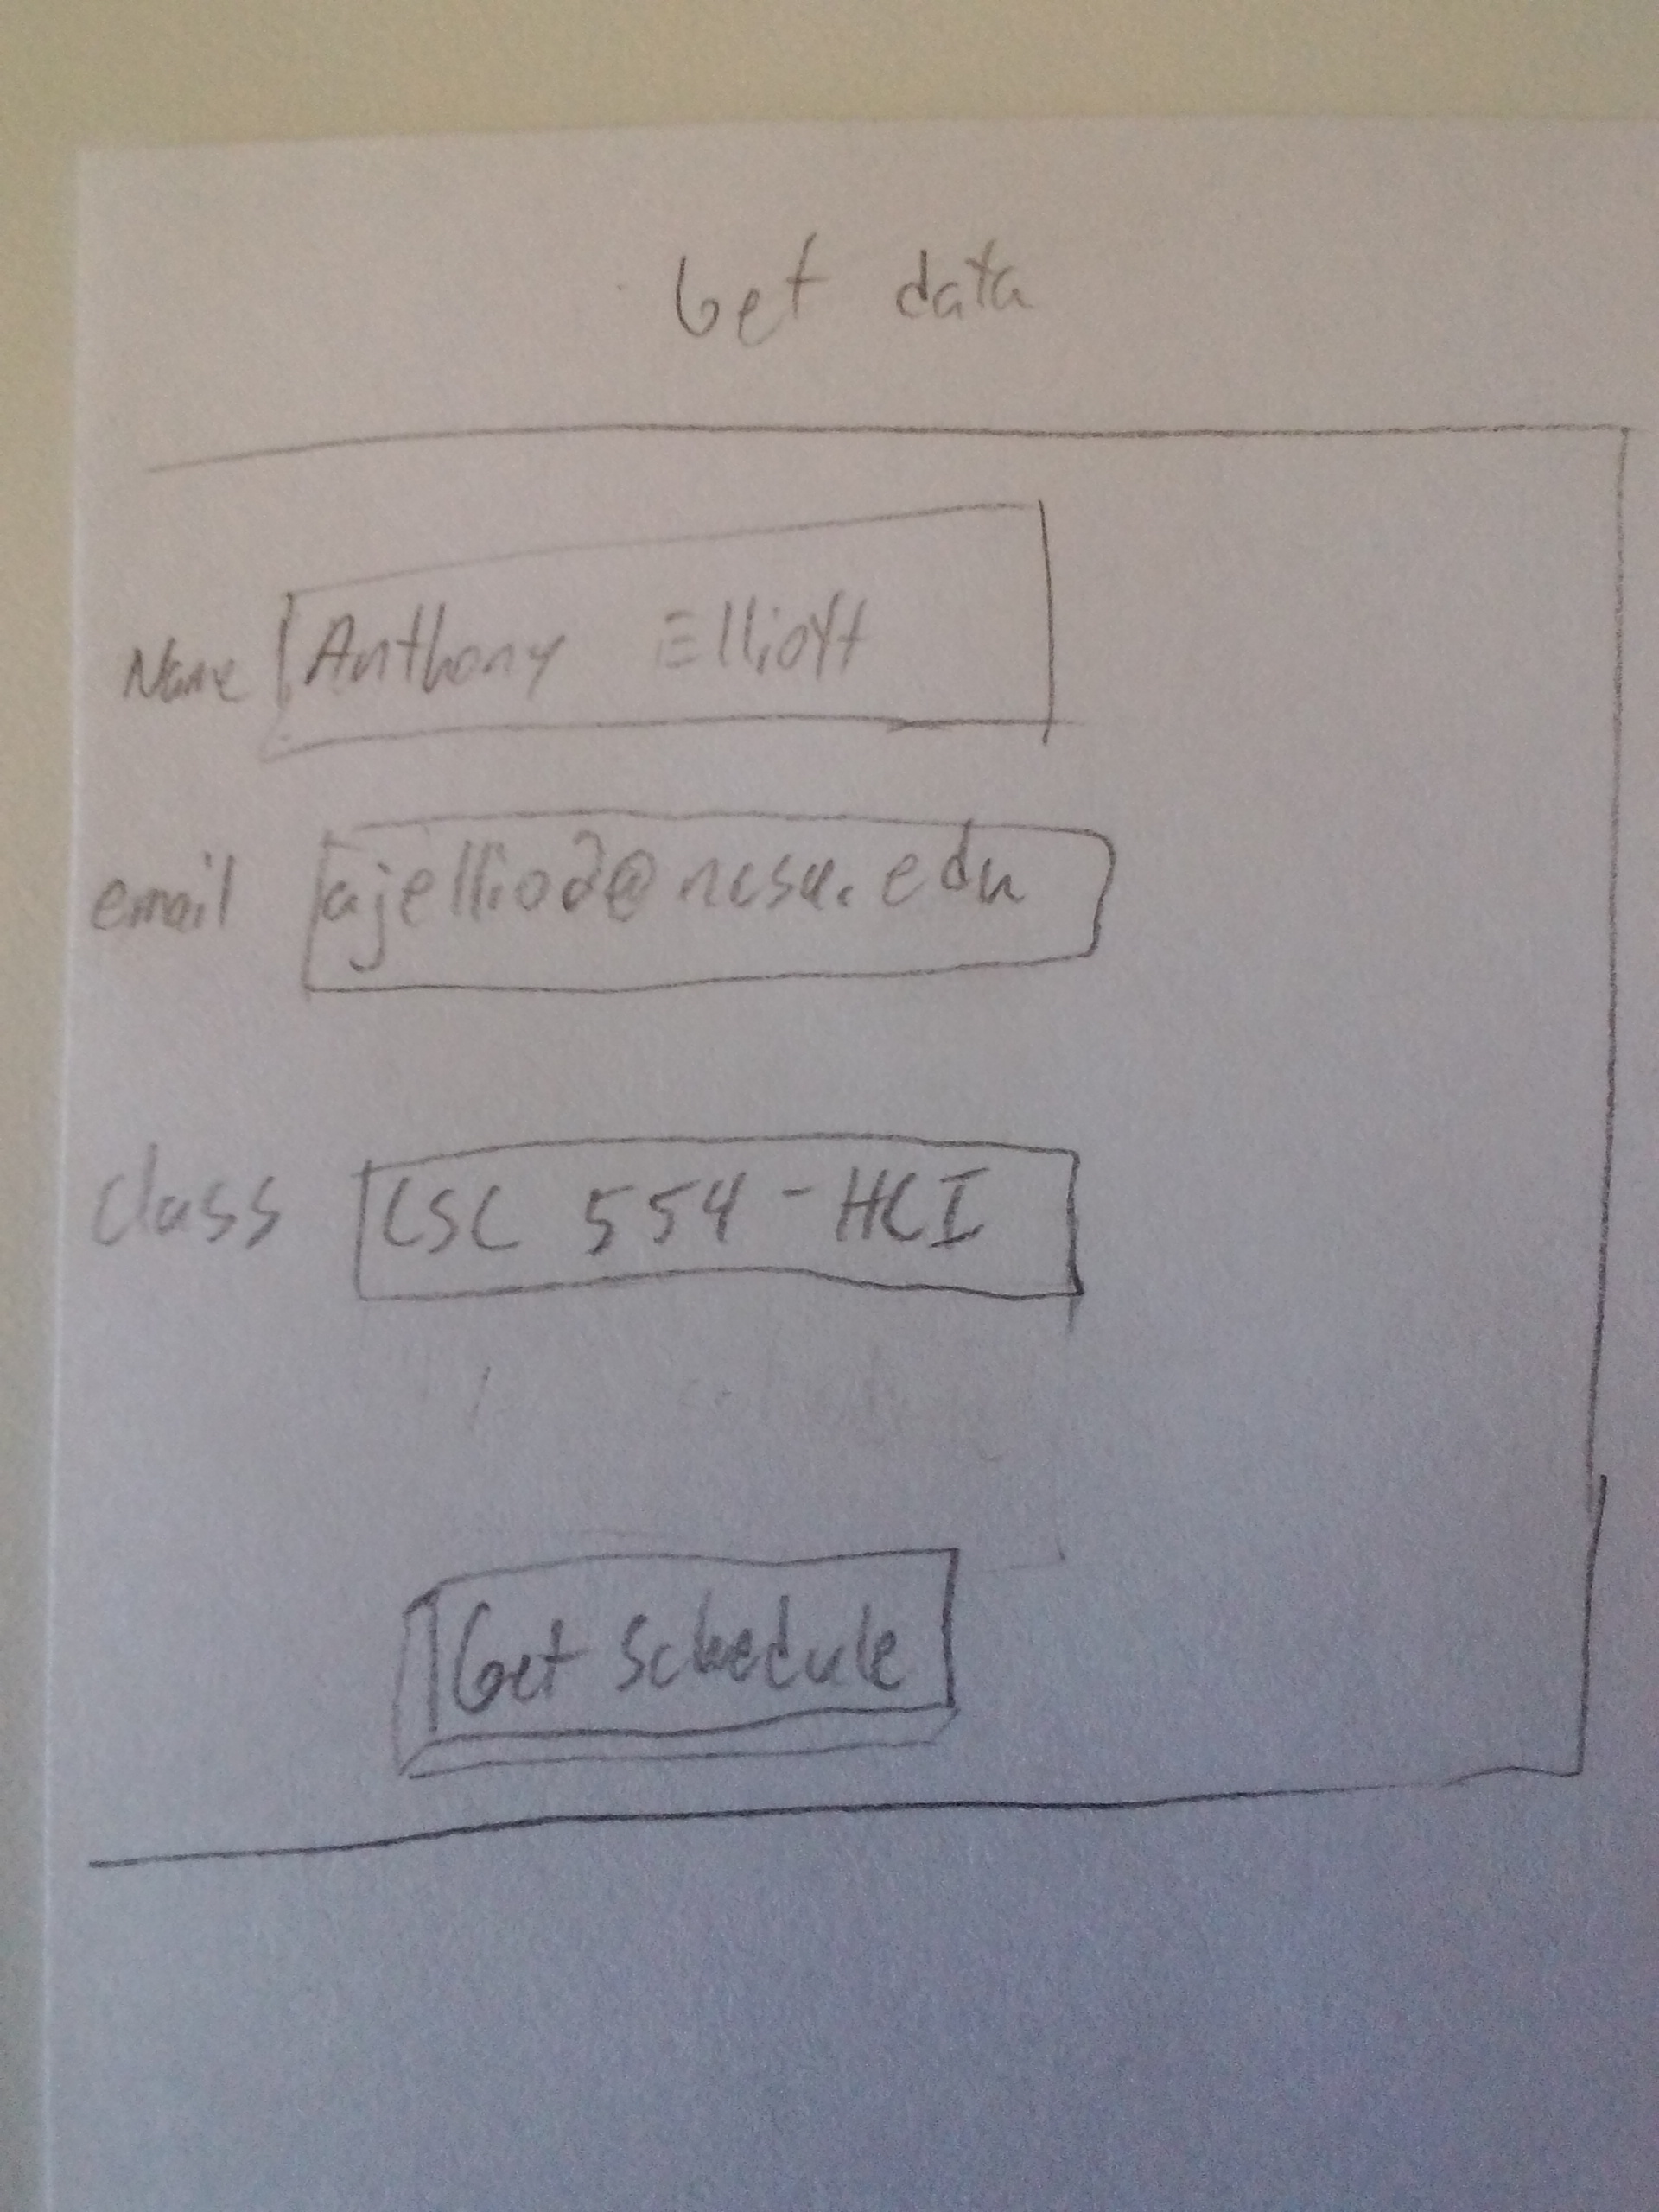
\includegraphics[width=80mm]{figures/getUserData}
\caption{Screen to get user data. \label{fig:userData}}
\end{figure}

\begin{figure}[ht!]
\centering
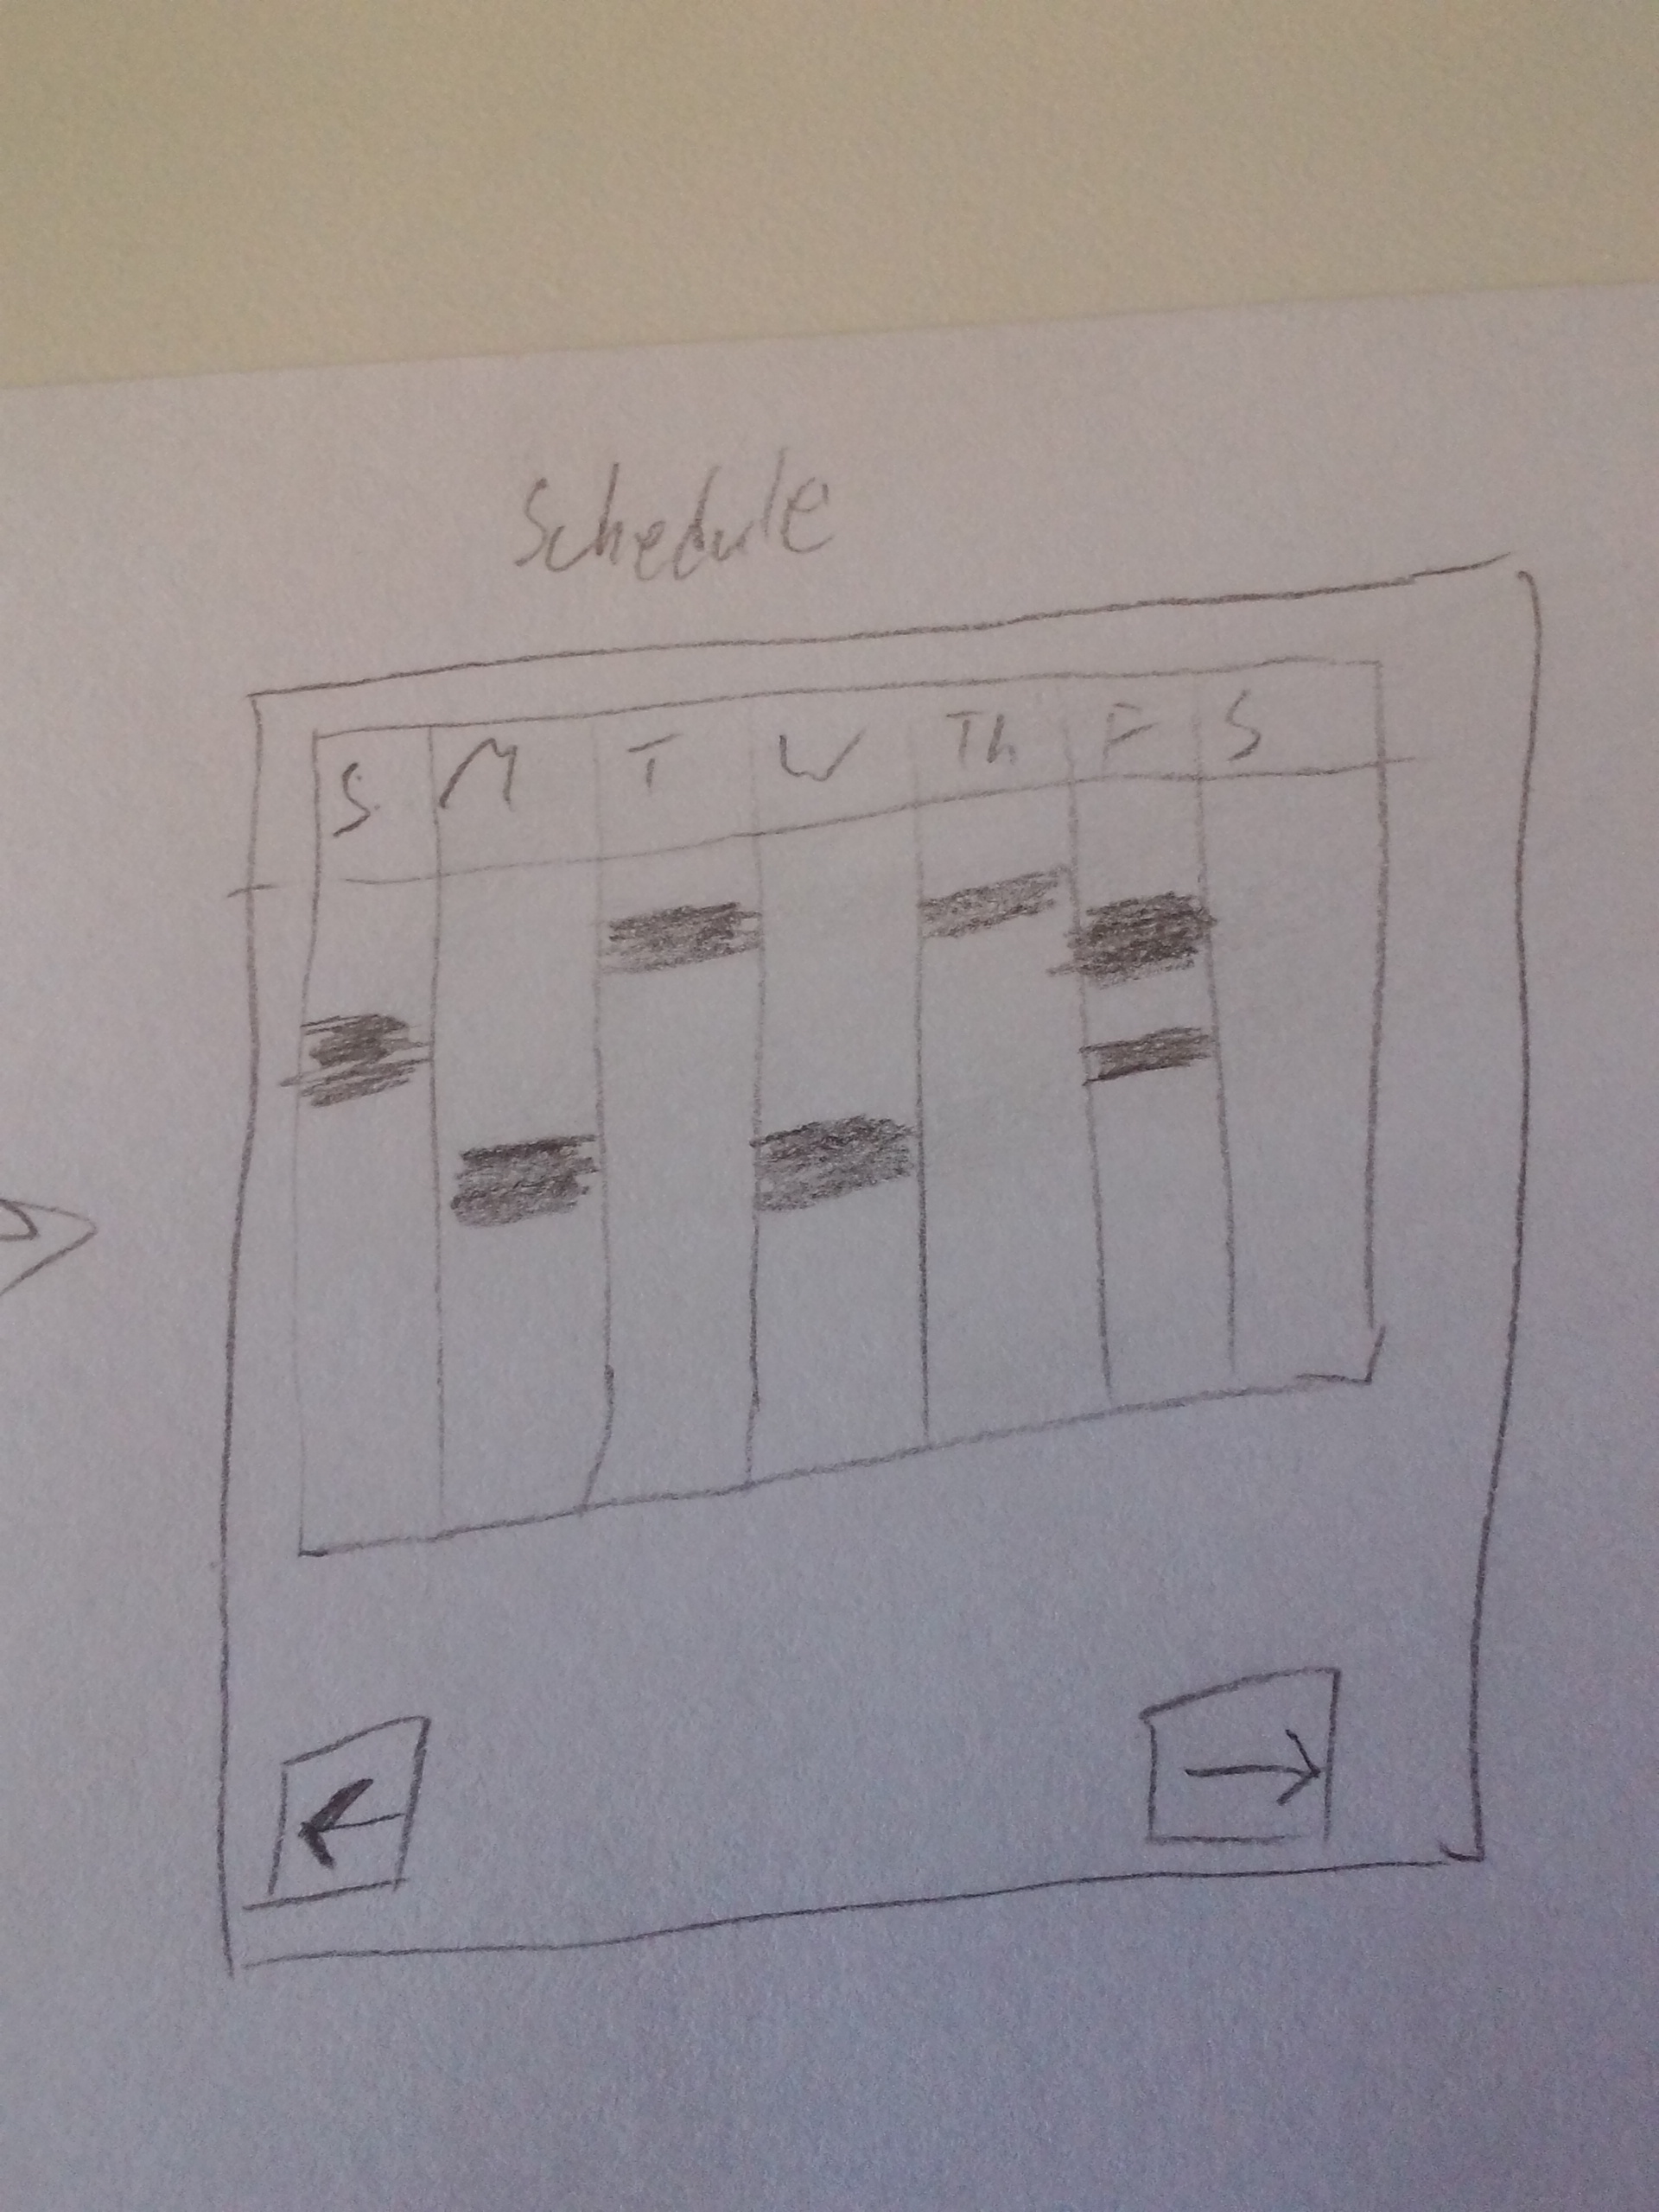
\includegraphics[width=80mm]{figures/schedule}
\caption{Shows the user's schedule. \label{fig:schedule}}
\end{figure}

\begin{figure}[ht!]
\centering
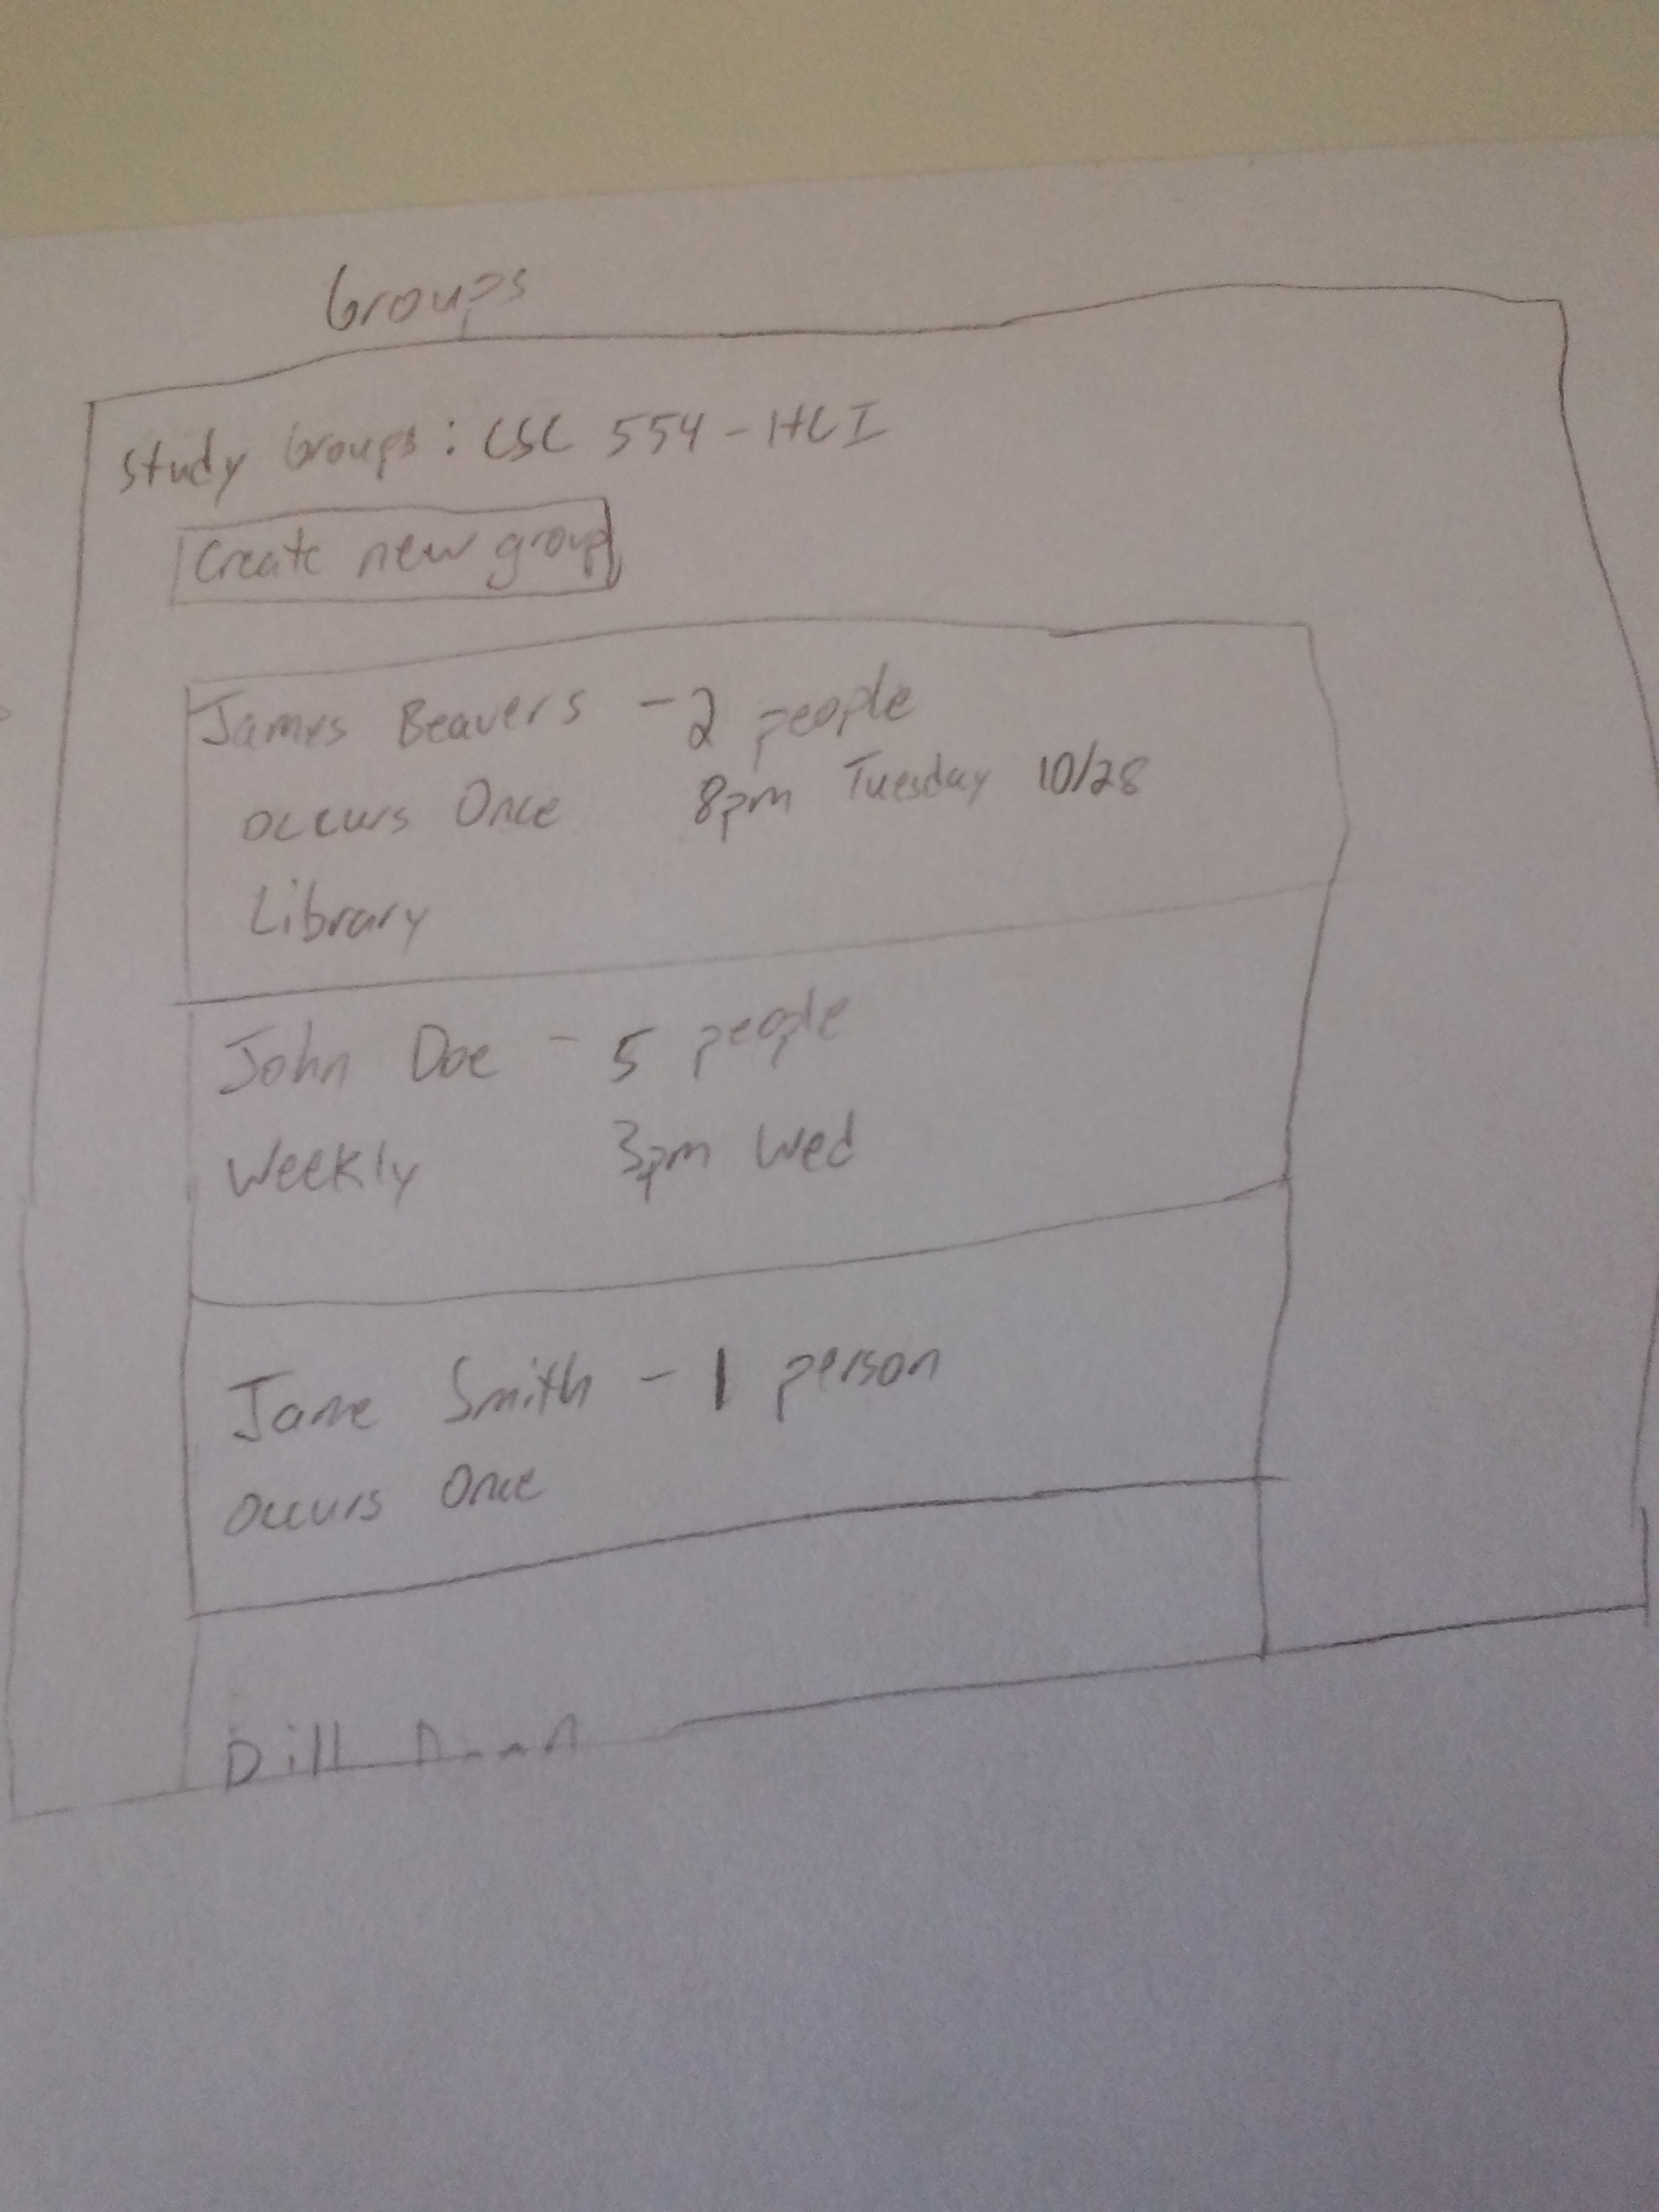
\includegraphics[width=80mm]{figures/groups}
\caption{Lists all groups. \label{fig:groups}}
\end{figure}

\begin{figure}[ht!]
\centering
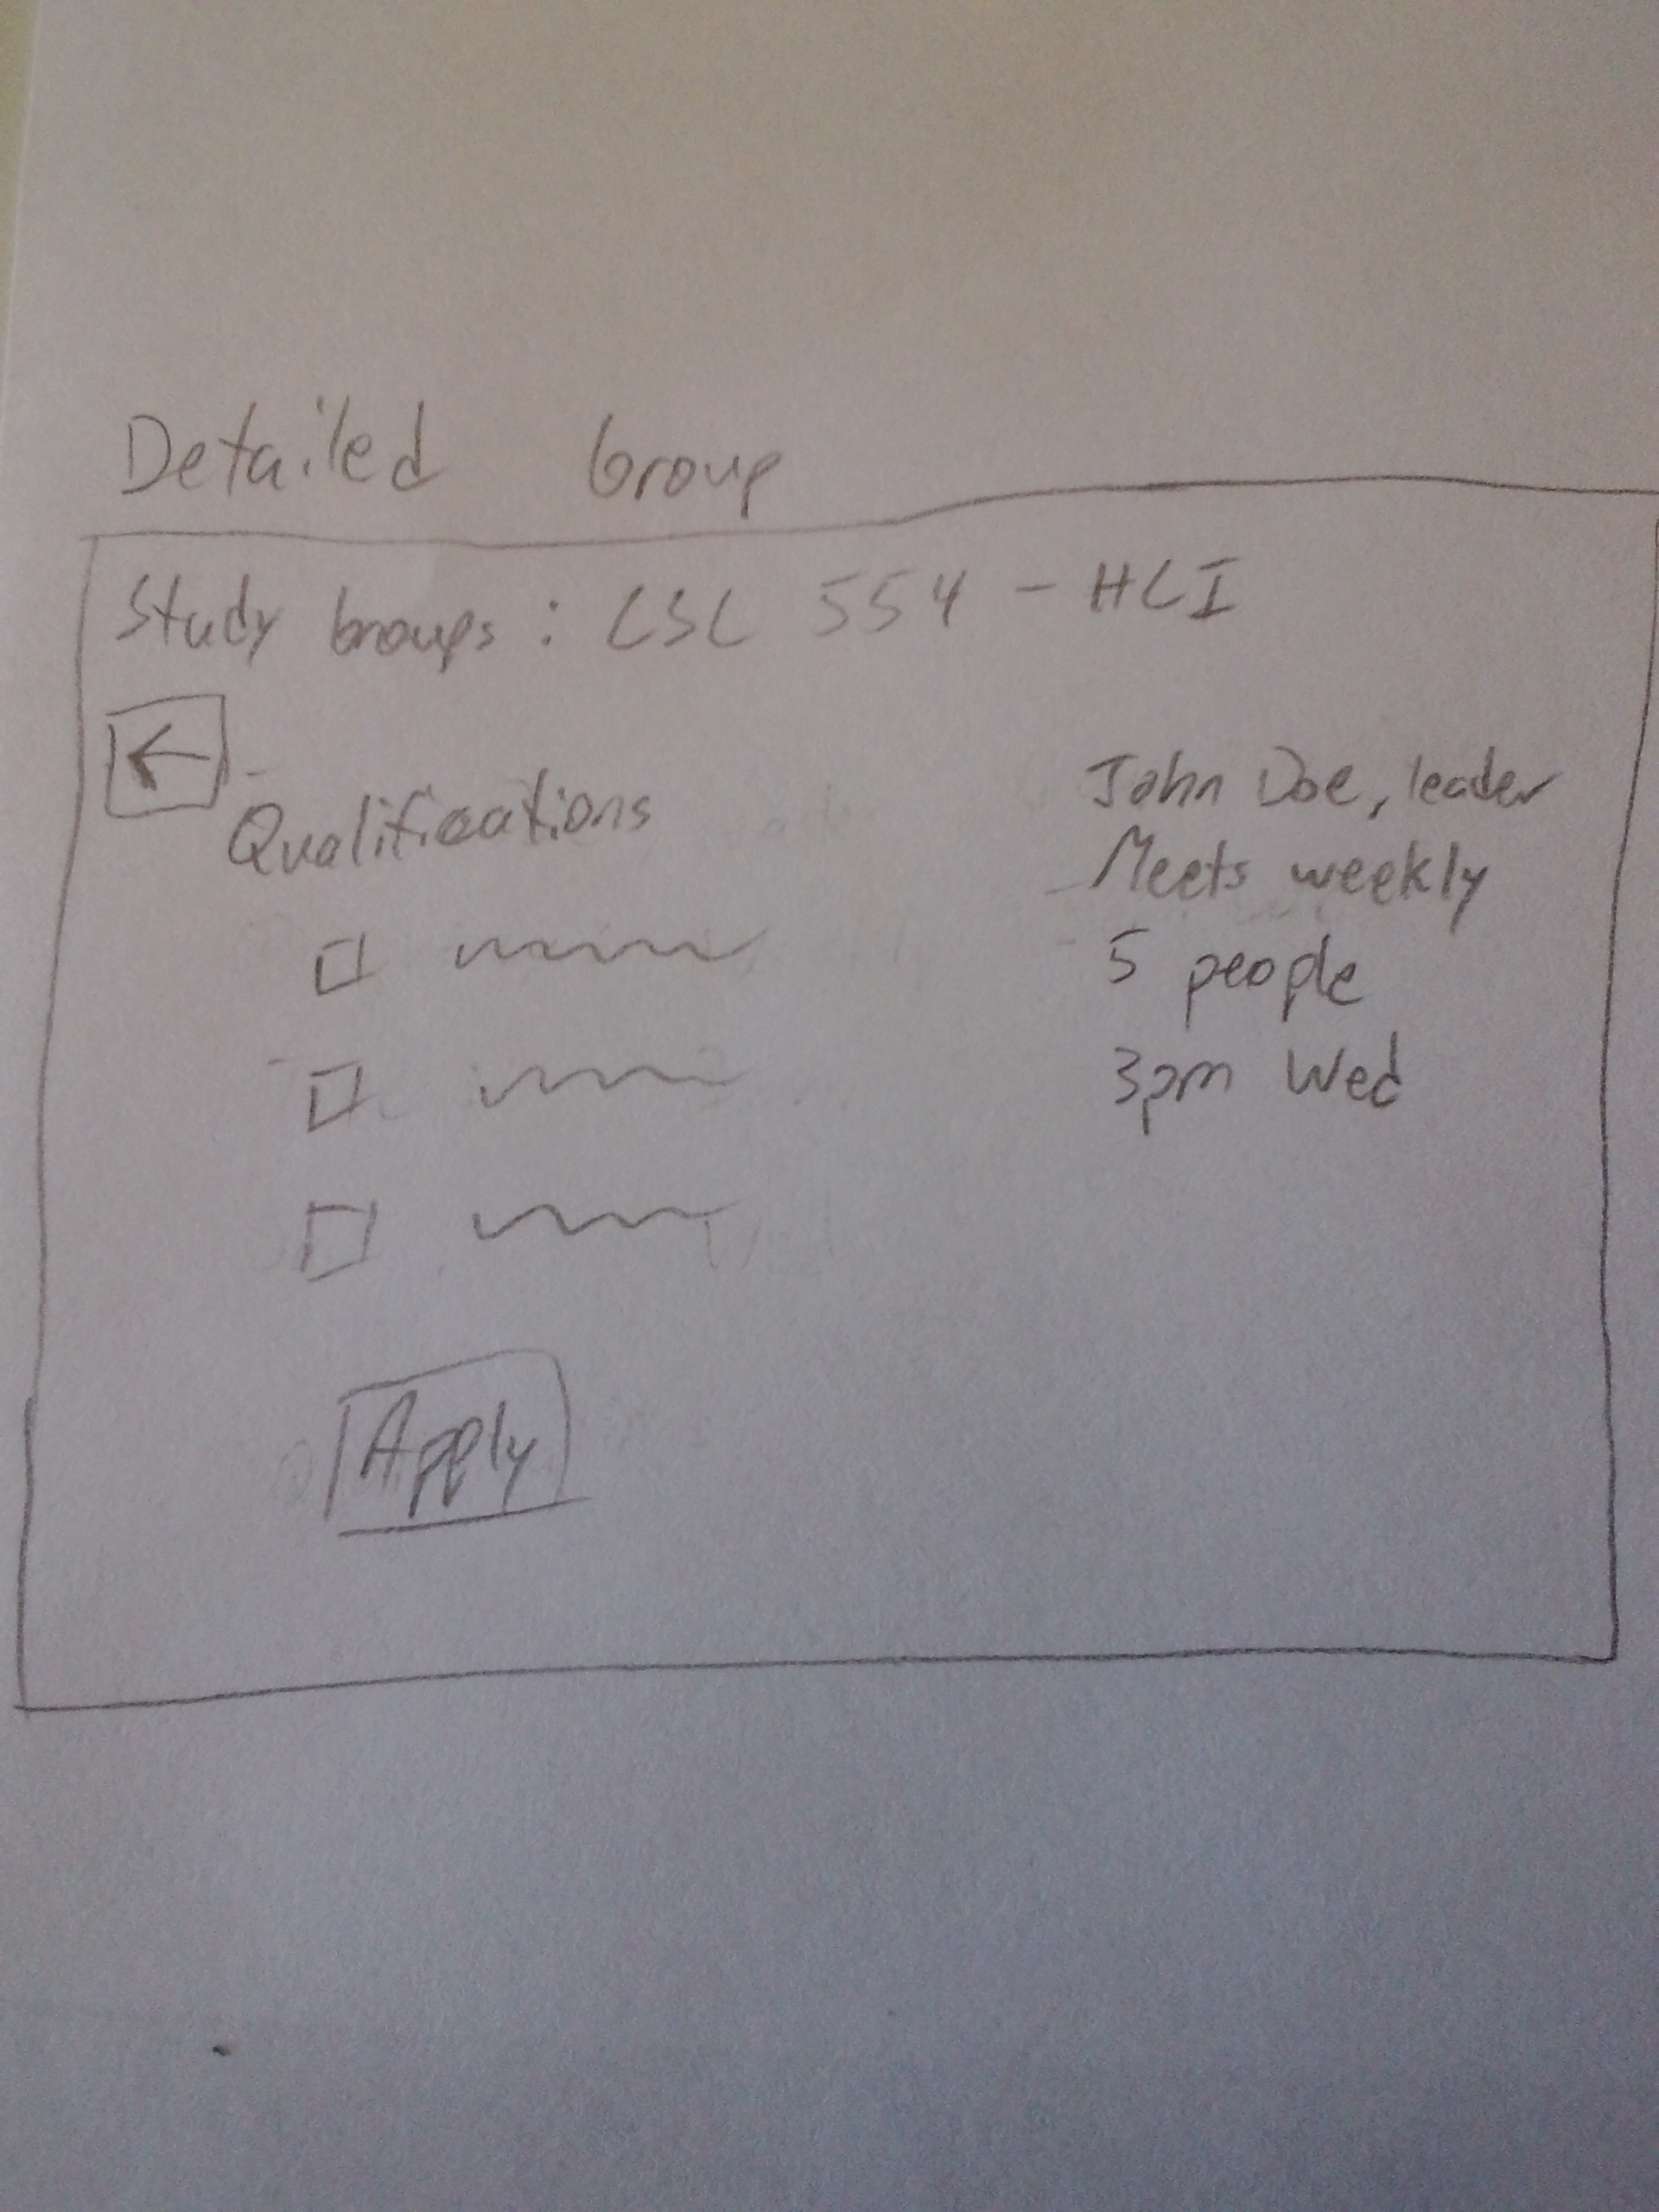
\includegraphics[width=80mm]{figures/detailedGroup}
\caption{Shows the detailed view of one group. \label{fig:detailedGroup}}
\end{figure}


\section{Interview Notes}
\textbf{Overview}
Looking at two different types of tools. One tool could be a `matchmaking' tool that helps to form the groups themselves. The other type is to assist study groups that have already been formed.

Neither of the interviewees thought that they would actually use a matchmaking tool. But they did like the tool that would assist the already formed group.

Could these two be combined?

Homework study groups are different than exam study groups.

\textbf{Details}
Helps to do bulk of the studying alone and then use SG to ensure people have the right understanding.

All participants should be at the same level

*helps to work examples together

everyone needs common background.
  are you comfortable with section x ?
  are you an expert on section y ?

personality.
  some people are really distracting and this completely undermines the entire study group.
  some people have an abnormally hard time understanding the material and would drag the group down.
  some people understand it very well and are a big asset to have in a SG.

Group size.
  Level of distraction increases with the number of people in the group.
  2 is ideal, 3 is ok, 4 is pushing it, 5 is almost always bad.
  distractions mean less efficient (more time spent in the group and less material covered well).
  also bad because people have different levels of understanding which slows the group down as a whole.

Length.
  depends on preparedness.
    is this an overview session or a teaching session?
  at least one hour, can last several hours.
      if night before exam then consider capping the session (one person didn't think this was as good of an idea on other nights).

using a study guide during the group is very helpful.
  cross off items as go through them.

If the group worked well then would likely use the same group later in the semester.
If group didn't work well then don't meet with other people again.

What about a way to rate the other people in the group after the session?  
Rate on how prepared they actually were, how much distraction they caused etc.

Sessions for exams are typically ad-hoc (only meet once, not regularly).

Groups are currently formed via friends / existing relationships.

Groups tend to not have leaders.  
Having one person in control means that the needs of other people likely will not be met.

Questions asked:
I asked several direct questions, but the subjects really got talking and covered a lot of the future questions without me needing to ask them.

I first explained what I was doing (interviews about study groups) and why (HCI project)
I opened with a very open-ended question:  Describe your past experiences with study groups
How often does the study group meet?
How many people typically come to the group?
Talk about how the group changes over the course of the semester.
How is the group run?  By one person, rotating leader, group leadership, etc.
How does the group communicate about group ideas outside of the group? (e.g. when the next meeting is, if meeting place/time changes)
What types of people make up your study groups--friends, project members, random study partners?
Are some study groups better than others?  What causes the differences?  Are these differences consistent?
Why do you go to study groups?
How do you form your study group(s)?

\bibliographystyle{abbrv}
\bibliography{bibliography}

\end{document}
